\chapter{绪论} \label{ch01}
科学计算分为数值计算和符号计算. 数值计算的输入输出和中间结果都是数值, 因为计算机对数值的存储精度有限, 所以数值计算是一种近似计算. 符号计算即为精确计算. 更广义的符号计算是指对代表数学对象的符号(包括整数\D 有理数\D 实数\D 复数\D 变量名\D 多项式\D 群\D 环\D 域\D 矩阵等)进行计算. 能够进行符号计算的软件被称为计算机代数系统. 常见的计算机代数系统有 Maple, Mathematica, Axiom, Maxima 和 Reduce 等. 计算机代数系统的出现, 为许多需要复杂的符号计算和推理的领域提供了有力的工具. 尤其是在求非线性系统精确解的相关研究中, 计算机代数系统更是不可或缺的工具. 本文对于非线性系统精确解的相关研究都是基于 Maple 平台完成的. 

\section{非线性演化方程的精确解}
非线性演化方程(Nonlinear Evolution Equations, 简称 NLEE)是描述自然界许多现象和内在规律的常用数学模型. 研究 NLEE 的精确解, 对我们了解事物的运动规律和科学地解释自然现象都具有重要的作用, 特别是在近代物理和科学工程计算中的一些关键问题, 都能归结为某些 NLEE 的求解问题. 

经过科研人员的不断努力, 发现了一系列求NLEE精确解的方法. 如反散射变换方法\cite{kawata1978inverse}\D Darboux 变换方法 \cite{matveev1991darboux}\D \Backlund{}变换方法 \cite{wahlquist1973backlund}\D 齐次平衡方法\cite{zhibin1993travelling}\D Hirota 方法 \cite{hirota1971exact}\D 混合指数方法\cite{hereman1986exact}\D 双曲正切方法\cite{malfliet1992solitary}\D Jacobi椭圆函数方法\cite{liu2001jacobi}等. 基于这些方法可以构造许多不同类型的精确解, 如孤子解\cite{hirota1971exact}\D 呼吸子解 \cite{tajiri1989breather}\D lump解\cite{satsuma1979two}\D 怪波解\cite{guo2011rogue}等. 下面我们主要对齐次平衡方法\D 双曲正切方法\D Jacobi 椭圆函数方法和 Hirota 方法进行简要介绍. 

(a) 齐次平衡方法

1993年, 王明亮和李志斌\cite{zhibin1993travelling}提出了求解NLEE行波解的齐次平衡方法, 并基于该方法构造了一些 NLEE 的精确解\cite{wang1995solitary,wang1996application}. 齐次平衡方法根据方程最高阶部分可部分平衡的原则, 确定方程的解应具有的一般形式, 再将这种形式代回原方程进行求解. 该方法是一种普适性方法, 已经被国内外许多学者用于求解各种方程的精确解\cite{hbm1998,senthilvelan2001extended,zhao2002new,rady2010homogeneous,nguyen2015modified}. 此外, 齐次平衡方法中确定解的阶数的思路被提炼为齐次平衡原则,一些机械化方法都是基于该原则发展起来的. 如\Painleve{}展开法\D 双曲正切方法和 Jacobi 椭圆函数方法等. 

(b) 双曲正切方法 

双曲正切方法始于黄国翔和楼森岳等人\cite{huang1989exact}的工作. 双曲正切方法将解假设为 tanh 函数的多项式, 基于齐次平衡原则确定解的阶数之后, 再通过待定系数法求解. 1992年, Malfliet\cite{malfliet1992solitary}系统地阐述了双曲正切方法. 1996年, Parkes 和 Duffy\cite{parkes1996automated}基于Mathematica 编写了 ATFM 软件包, 基本实现了双曲正切方法的自动化. 2002年, 李志斌和柳银萍\cite{liu2001master,li2002rath}在 Maple 上编写了 RATH 软件包,完全实现了双曲正切方法. 同时, 他们还首次引入了一个变换, 可以在平衡次数不是正整数的时候获得关于 tanh 函数的有理函数解. 2004年, Maple 9.5 \footnote{\url{https://www.maplesoft.com/support/help/Maple/view.aspx?path=updates/Maple9_5/de}}在 PDEtools 库中嵌入 TWSolutions 函数来实现双曲正切方法. 同时, Wazwaz\cite{wazwaz2004tanh}\D Abdou\cite{abdou2007extended}\D 范恩贵\cite{fan2000extended}\D 张鸿庆\cite{lu2003further}\D 陈勇\cite{zheng2003generalized}和闰振亚\cite{yan2001new}等人也对双曲正切方法进行了一些拓展和应用. 

(c) Jacobi椭圆函数方法

2001年, 刘式适等人\cite{liu2001jacobi}将双曲正切函数法中的 tanh 函数替换为 Jacobi 椭圆函数, 提出了 Jacobi 椭圆函数方法. 2002年, 柳银萍和李志斌\cite{yin2002automated}研发了软件包 AJFM, 实现了 Jacobi 椭圆函数方法的完全自动化. 2004年, 他们\cite{li2004raeem}又研发了软件包 RAEEM, 该软件包可以完全自动地推导出 NLEE 不同类型的行波解, 包括多项式解\D 指数函数解\D 三角函数解\D 双曲函数解\D 有理函数解\D Jacobi 椭圆函数解和 Weierstrass 椭圆函数解. 2005年, Maple 10 \footnote{\url{https://www.maplesoft.com/support/help/maple/view.aspx?path=updates/Maple10/de}}在 PDEtools[TWSolutions] 中集成了相关功能. 同时, 周宇斌\cite{zhou2003periodic}\D 范恩贵\cite{fan2002applications}\D 张解放\cite{jia2004general,chao2005symbolic}\D 陈怀棠\cite{chen2003improved}\D 张鸿庆\cite{yu2005extended}\D 徐桂琼\cite{gui2005applications}\D 陈勇\cite{chen2005extended}\D Abdou\cite{abdou2007construction} 和 Bhrawy\cite{bhrawy2013cnoidal}等人也对 Jacobi椭圆函数方法进行了拓展和应用. 

(d) Hirota 方法

Hirota 双线性方法是由日本数学家 Hirota\cite{hirota1971exact}于1971提出的, 该方法思路简单\D 适用范围广, 后被众多学者应用和推广. 1973年, Hirota\cite{hirota1973exact}在求解浅水波的孤子解时, 将多孤子解的生成公式重写, 该形式被后来的研究者们广泛接受.  基于 Hirota 方法不仅可以构造 NLEE 的多孤子解, 还能构造出其它类型的解. 
1979年, Satsuma 和 Ablowitz\cite{satsuma1979two} 在 Hirota 方法的基础上提出了长极限方法, 获得了(2+1)维 KP 方程\cite{kadomtsev1970stability}的 lump 解. 
1981年, Hirota 和 Ito \cite{hirota1983resonance}利用 Hirota 方法得到了孤子方程的共振解. 
1989年, Tajiri等人\cite{tajiri1989breather}基于 Hirota 方法提出了共轭参数法, 能够从多孤子解得到呼吸子解. 
1990年, Hietarinta \cite{hietarinta1990multidromion} 利用 Hirota 方法得到了 Davey-Stewartson 方程的 Multidromion 解. 
1997年, Lambert 等人\cite{gilson1996combinatorics,lambert1997construction} 将 Bell 多项式和 Hirota 方法结合起来, 拓展了Hirota 方法的应用范围. 
Wazwaz\cite{wazwaz2008multiple}\D 范恩贵\cite{fan2011new}\D 胡星标\cite{hu2002application}\D 陈登远\cite{chen2002novel}和张大军\cite{zhang2003n}等人也对 Hirota 方法进行了许多的推广和应用. 
\mk{近年来, Hirota 方法也被用于求怪波解\cite{guo2011rogue,sun2018general,zhaqilao2018symbolic}.}{Lump 就不重复引用了, 反正讲过了, 不引用也没事}

关于 Hirota 方法的机械化实现也有一些优秀的工作. 1992年, Hereman 等人\cite{hereman1992symbolic,hereman1991macsyma} 简化了 Hirota 双线性方法, 提出了简单 Hirota 方法, 并在 Macsyma 上进行了实现, 该程序能够处理KdV型双线性方程. 2012年, 周振江\cite{zhou2012}在Maple上实现了 Hirota 双线性方法的相关软件包 Bilinearization 和 Multisoliton. 其中 Bilinearization 能够将 NLEE 双线性化, Multisoliton 能够求得多孤子解. 此外, 还有杨云青\D 苗倩和陈勇等人\cite{yang2011,miao2014pdebellii}在 Lambert 等人工作的基础上, 结合 Hirota 方法和 Bell 多项式, 实现了 PDEBell 和 PDEBellII 软件包, 能够自动推导 KdV 类和 mKdV 类方程的孤子解. 

\section{非线性差分方程的精确解}
求差分方程的精确解也是计算机代数的重要研究内容. 差分方程有时也被称为递归方程. 最简单的差分方程是线性常系数差分方程, 即
\begin{equation}
\sum_{k=0}^l{c_k f(x+k)}=g(x),
\label{ceq}
\end{equation}
其中 $f(x)$ 是未知函数, $g(x)$表示任意多项式, 而$c_k (k=1,\cdots,l)$是任意常数. 该方程的求解在很久以前就已经被解决了. 我们可以简单地将\refeqnn{ceq}拓展为线性多项式系数的方程
\begin{equation}
\sum_{k=0}^l{p_k(x)f(x+k)=p_{l+1}(x)}, 
\label{peq}
\end{equation}
其中 $p_k(x) (k=1,\cdots,l+1)$是多项式. 1989年, Abramov\cite{Abramov1989polynomial}首先考虑了该方程, 提出了求解多项式解的算法. 同年, Abramov\cite{Abramov1989rational}又提出了寻找所有有理函数解公分母的算法, 从而提出了求有理函数解的算法. 1992年, \Petkovsek{}\cite{petkovvsek1992hypergeometric}提出了求解超几何函数解的算法. 超几何函数相邻两项之比是有理函数. 在超几何函数解上进行移位和部分和操作能够生成 d'Alembertian 解. d'Alembertian 解的求解算法是在1994年由 Abramov 和 \Petkovsek{} \cite{abramov1994dAlembertian}共同提出的. 在 d'Alembertian 解上执行移位\D 部分和以及交错操作能够得到 Liouvillian 解. Liouvillian 解的求解算法是1999年由 Hendricks 和 Singer \cite{hendricks1999Liouvillian}提出的.

虽然在 Liouvillian 解之后并没有找到更一般的解, 但是\refeqnn{peq}的求解算法还在不断改进. 一些改进是将这些算法推广到q-差分方程和微分方程. 例如\citett{Abramov1995polynomial}是对多项式解的推广应用, \citett{Abramov1995Rational} 是对有理函数解的推广应用. 另一些改进是为了提高算法的效率. 例如, \citett{ud2007,ud2010,ud2011,ud2012} 是一系列对有理函数解公分母求解算法的改进. 因为这一步是有理函数解求解过程耗时最长的一步, 所以这些改进极大地提高了有理函数解的求解效率. 

目前, 关于线性差分方程的研究成果较多, 而关于非线性差分方程的研究则较少, 只有几类特定方程的相关研究\cite{chen2011some,ishizaki2011difference}. 因此, 本文将研究一般非线性差分方程的求解. 

\section{非线性积分化简}
\red{
在求微分方程的精确解时, 往往离不开符号积分. 例如, 在求双线性形式的过程中需要对奇次表达式积分一次并化简, PDEBellII在开发过程中就未能完全解决该问题\cite{miao2014}.
}

符号积分也是计算机代数的一个重要组成部分. 在符号计算的发展初期, 就有关于基本初等函数符号积分的相关研究. 最早的符号积分软件SAINT\spell{(Symbolic Automated INTegrator)}和SIN\spell{(Symbolic INtegrator)}分别发表于1963年\cite{slagle1963}和1967年\cite{moses1967}. 符号积分中最重要的基础算法是Risch算法\cite{risch1969,risch1970}, 它是近几十年来符号积分发展的基础. 在 Risch 算法发表后不久, Moses 在 SIN 的改进版本中首次实现了纯超越函数的部分\cite{moses1971}. 而 Bronstein 则在 1990 年\cite{bronstein1990} 对基本初等函数的一般情况进行了实现. 几乎所有的计算机代数系统(如 Maple, Mathematica, Axiom, Maxima 和 Reduce 等), \red{都是以 Risch 算法为基础来计算符号积分的.} 

当基本初等函数的符号积分被解决以后, 科研人员主要致力于特殊函数符号积分的研究\cite{cherry1985,cherry1986,bertrand1994,jeffrey1997}. 近年来, 关于特殊类型的符号积分研究较多, 如相对论库伦积分\cite{paule2012,paule2013}\D Feynman积分\cite{blumlein2012,smirnov2015}和参数积分\cite{raab2016}等.

然而, 关于抽象函数的积分的研究却很少, 只有\citett{deconinck2009}和\citett{poole2010}提出了一个算法来寻找线性可积的抽象函数表达式的积分. 他们的算法主要致力于寻找方程$D_x f=g$的解. 其主要作用是寻找偏微分方程中的守恒律\cite{poole2011}, 而不是计算一般的抽象函数积分表达式. 因此, 本文将抽象函数积分表达式的化简作为一个具有挑战性的课题进行研究.

\section{本文的选题和主要工作}
随着计算机代数系统的不断发展, 衍生了许多构造非线性系统精确解的机械化方法. 本文在前人工作的基础上, 针对非线性系统精确解的相关机械化算法进行研究, 开展了如\reffig{outline}所示的一些工作. 在\reffig{outline}中, 椭圆表示方法\D 矩形表示软件包. 其中 矩形内部的第一行是软件包的名称, 第二行是软件包用途的简要说明. 软件包以4种颜色进行区分, 黄色表示基础工具, 蓝色表示用于求解差分方程, 绿色表示用于求解微分方程, 粉色表示用于进行积分化简. 

\begin{figure}[htbp]
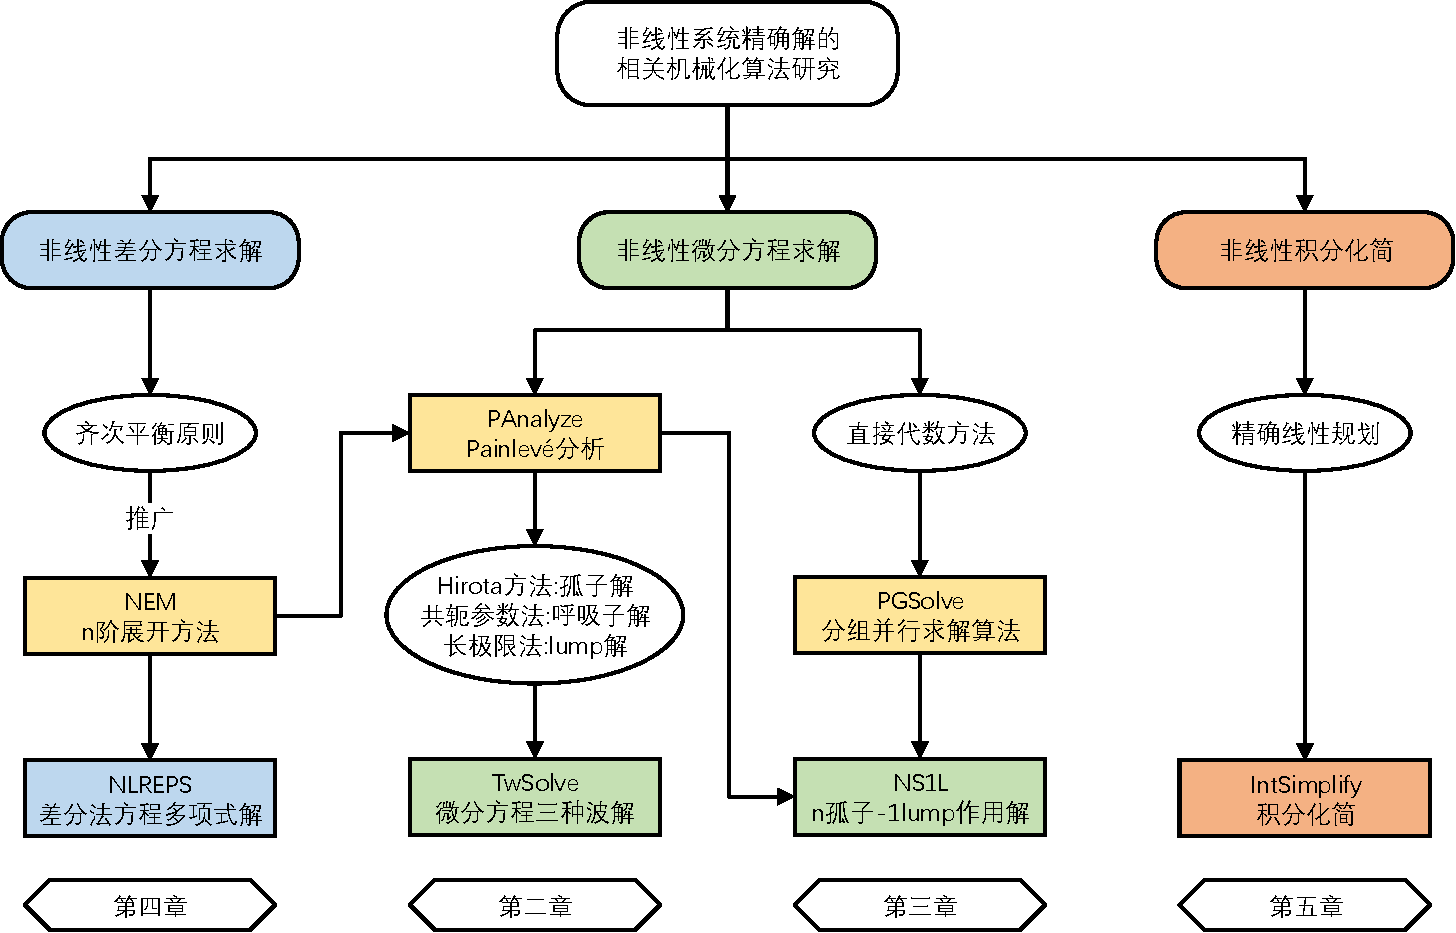
\includegraphics[width=\textwidth]{fig/outline.pdf}
\caption{本文工作大纲图}\label{outline}
\end{figure}

\red{
在\refchp{ch02}中, 因为由 Hirota 方法推导出的$n$孤子解公式只对可积方程成立, 本文引入了一种参数约束条件, 将$n$孤子解公式推广到不可积方程的情形. 基于简单Hirota 方法\D 共轭参数法和长极限法, 发展出了构造非线性演化方程的孤子解\D 呼吸子解及 lump 解的机械化算法, 研发了相应的软件包 TwSolver, 并在编程实现时对上述方法的一些细节进行了优化. 
}

直接代数方法在微分方程的求解中也有广泛的应用, 它的主要难点是其中大规模非线性代数方程组的求解. 在\refchp{ch03}中, 本文针对大规模非线性代数方程组求解困难的问题, 设计了一个分组并行的求解算法, 研发了相应的软件PGSolve. 作为 PGSolve 的应用实例, 本文开发了用直接代数方法求$n$-孤子和1-lump相互作用解的软件包 NS1L. 

在\refchp{ch04}中, 本文将齐次平衡原则推广为$n$阶展开方法, 并将其应用于微分方程和差分方程的若干求解方法中. 求解微分方程的许多方法都是基于齐次平衡原则发展起来的, 如\Painleve{}展开法\D 双曲正切方法和 Jacobi 椭圆函数方法等. 这些方法通常都是将方程的解假设为某个函数的多项式, 通过平衡方程中两个不同最高项的阶数来确定解的阶数. 但是, 当一个方程的各个最高次项的阶数的表达式相同时, 则根据齐次平衡原则没法确定解的阶数的上界, 从而有可能漏解. 本文发现, 解的阶数不仅会出现在最高$n$项的阶数中, 还会出现在最高$n$项的系数中. 因此, 本文考虑同时平衡方程中最高$n$项的阶数和系数, 提出了$n$阶展开方法, 研发了 NEM 软件包. 基于$n$阶展开方法, 我们提出了一个求解非线性差分方程多项式解的新算法, 并研发了相应的软件 NLREPS. 同时, 本文还将$n$阶展开方法应用于双曲正切方法和\Painleve{}展开法中. 

在\refchp{ch06}中, 因为在非线性微分方程的求解过程中往往需要进行积分表达式的化简, 本文将抽象函数的非线性积分化简作为一个具有挑战性的任务进行研究. 首先, 本文建立了一个代数系统将关于抽象函数的积分多项式视为标准积分项的线性组合. 然后, 基于导数的乘法规则, 设计了一个递归算法来寻找所有的二项合并规则. 最后, 基于这些规则将化简问题转化为一个精确线性规划问题进行求解, 实现了非线性积分表达式化简的软件包 IntSimplify.  

\refchp{ch07}对本文完成的工作进行了总结与讨论,概括了本文的主要研究方法和结论,并对未来的工作提出了展望.

需要说明的是, 本文的主线是非线性微分方程精确解的构造算法及其机械化的研究. 非线性差分方程多项式解的构造算法及其机械化研究是$n$阶展开方法的推广应用; 而抽象函数的积分多项式化简是为微分方程的化简和求解提供一个辅助工具. 
